\documentclass[a4paper,11pt]{article}

\usepackage[margin=3cm]{geometry}

\usepackage{graphicx}
\usepackage{subcaption}
\usepackage[colorlinks,allcolors=violet]{hyperref}
\usepackage{url}
\usepackage{lmodern}

% https://tex.stackexchange.com/questions/94032/fancy-tables-in-latex
\usepackage[table]{xcolor}
\usepackage{booktabs}

\usepackage[utf8]{inputenc}

% https://tex.stackexchange.com/questions/664/why-should-i-use-usepackaget1fontenc
\usepackage[T1]{fontenc}
\usepackage{microtype} % good font tricks

\newcommand{\note}[1]{{\colorbox{yellow!40!white}{#1}}}
\newcommand{\exampletext}[1]{{\color{blue!60!black}#1}}

\begin{document}

\noindent
\colorbox[HTML]{52BDEC}{\bfseries\parbox{\textwidth}{\centering\large
  --- Report P\&O CW 2019--2020 Task 3 ---
}}
\\[-1mm]
\colorbox[HTML]{00407A}{\bfseries\color{white}\parbox{\textwidth}{
  Department of Computer Science -- KU Leuven
  \hfill
  \today
}}
\\

\smallskip

\noindent
%\mbox{}\hfill
\begin{tabular}{*4l}
\toprule
\multicolumn{2}{l}{\large\textbf{Team 12}} \\
\midrule
Toon Sauvillers & 60h \\ % fill in the time spend on this task per team member who worked on it
Seppe Van Steenbergen & 54h \\
Bert Van den Bosch & 52h \\
Frédéric Blondeel & 20h \\
\bottomrule
\hline
\end{tabular}\\

\noindent
{\color[HTML]{52BDEC} \rule{\linewidth}{1mm} }

\section{Introductie}\label{sec:introductie}
Het herkennen van schermen, deze identificeren, lokaliseren uit een foto. Dit verslag behandeld deze uitdagingen. Het zoeken van schermen begint bij een foto. Deze foto bevat een scherm met een bepaald uitzicht, er is gekozen voor een groen-blauwe rand waarop gefilterd kan worden. Vervolgens zoekt het algoritme in de gefilterde foto naar aparte schermen en geeft aan hen een id. Met behulp van het kleurenverschil en bepaalde hoeken wordt de oriëntatie bepaald.

Het identificeren van het scherm gebeurd op dit moment nog apart met een kleurenbarcode. Deze barcode bevat 5 verschillende kleuren waardoor er 120 verschillende schermen geïdentificeerd kunnen worden. In de volgende weken worden deze twee, lokaliseren en identificeren, bij elkaar gezet.
\\
Dit verslag behandeld de keuzes die gemaakt zijn alsook een uitleg bij de gebruikte algoritmen en hun tijdscomplexiteit. De mogelijke beperkingen worden met deze kennis geduid.
% The communication protocol should accommodate for:
% \begin{itemize}
%     \item The transmission of images from the smartphone camera to the master.
%     \item Manipulation of the background color of the client screens.
% \end{itemize}
% We are developing a game that requires two players who engage in a confrontation to take a mug shot picture of each other.
% Our game rules will positively encourage both players to provide clean pictures.
% This turned out to be essential since the DeepFace neural network \cite{website:facerecognizer} that we use was not accurate enough in the other scenario's we tested.
% Our analysis of the recognition rate is given in \S\ref{sec:technical-analysis}. Our systematic tests showed we have less than $1\%$~probability of not identifying the correct user out of our test database with $1000$ representative mugshot pictures.

% One unforeseen side effect of the usage of the DeepFace~\cite{amos2016openface} algorithm is the high power consumption.
% We had to balance the performance of the face recognition with battery life time. This was most significant for our indoor game play. In a test run we estimated that the average mobile phone from the supported types will be capable of playing for about $4$~hours and in that time frame scanning and identifying $60$~pictures per hour, see \S\ref{sec:technical-analysis}.
}

\section{Design schematics and screenshots}\label{sec:schematic}

\note{($\approx$ 1 page. Depending on the need for a design overview.)}
\exampletext{\textit{Design schematics, deployment diagrams, class diagrams, sequence diagrams, \ldots\ Whatever you think we need to understand your design. You could add a little bit of text here but keep that under half a page. You reference the illustrations here from~\S\ref{sec:technical-analysis} when needed.}}

\exampletext{All communication between clients runs through a nodejs server. We use the Socketio~\cite{socketio} library to set up a bidirectional communication channel between client and server. A deployment diagram can be found in Figure~\ref{fig:deployment}. Clients can take on a specific master or slave role by opening a specific webpage within the browser, i.e., the slaves will surf to \texttt{webaddress/slave}, while a client that wants to be the master loads the webpage found at \texttt{webaddress/master}.}

\begin{figure}[h!]
	\centering
	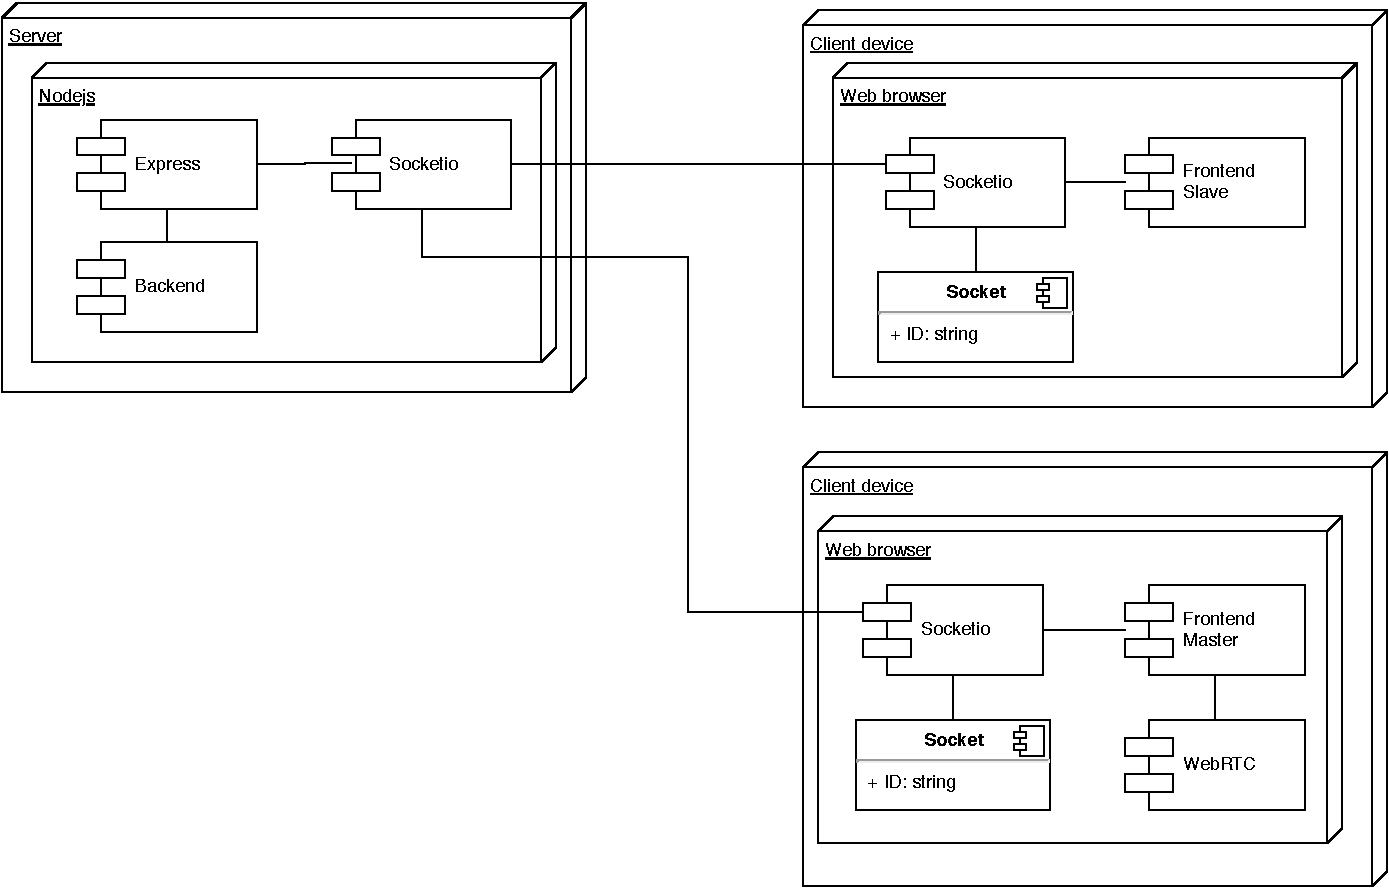
\includegraphics[width=\textwidth]{figures/deployment}
	\caption{Deployment diagram of the multiscreen casting framework.} 
	\label{fig:deployment}
\end{figure}

\exampletext{We rely on webrtc~\cite{website:webrtc} to collect a client-side video stream. This module offers the necessary tools for serialization, i.e., as a base64 encoded string. Serialization is required for transmission~\cite{website:serialization}. Server-side the backend code will process the image. In our demo we broadcast the image by sending it to all slaves. Slaves and masters can be reached by the server, as we use the concept of a namespace~\cite{website:namespaces}. A namespace can be used to group clients with a similar role, and broadcast to them. 

A socket is assigned a unique identifier by Socketio. This identifier can be used to emit messages from the server to a specific client. A list of connected clients is available through the API of Socketio \cite{website:socketio-clients}.}

\section{Algorithms}\label{sec:technical-analysis}

\note{($\approx$ 1 page. Depending on necessity)}
\exampletext{\textit{When you design or use an algorithm you should be able to explain how well it performs and if it satisfies the requirements. Often there will be alternatives or system parameters that need to be chosen. We want to know why you chose a specific set of parameters, or why you chose an approach over another. We supply some example text of last year.}}



\subsection{Scherm identificatie met barcodes}

\subsubsection{Algemene uitleg}

De identificatie van schermen gebeurt aan de hand van een kleuren barcode. Het slave-scherm zal binnen zijn rand(gebruikt voor edge detection) een herhalend patroon van 5 kleuren en wit tonen. Aan de hand van de volgorde kan een unieke code per scherm gelezen worden en zo is elk scherm duidelijk gedefinieerd. De 5 kleuren zijn speciaal gekozen om zo ver mogelijk uit elkaar te liggen in het HSL spectrum om fouten lezingen te vermijden. Ze dragen elk een cijfer van 1 tot en met 5 en worden maar één keer gebruikt in de barcode. Dit zorgt ervoor dat we in theorie een totaal van $5!$ ($=120$) verschillende schermen op één moment kunnen detecteren. Het herhalend patroon geeft ons de mogelijkheid om fouten te vermijden. Na het vinden van het scherm zelf (zie sectie 3.2) zal de barcode gelezen worden. Indien een reflectie of een overlap plaatsvind kan een stuk van het scherm bedekt zijn. De scanner() zal het midden van het scherm lezen in rechte lijn (volgens de orientatie), aangezien een stuk bedekt is zal deze blijven gaan tot hij 5 kleuren en wit tegenkomt. Zo niet, zal de lijst met codes leeggemaakt worden en verder gaan. Het herhalend patroon is dus essentieel aan het correct inlezen.

\begin{figure}
\centering

\includegraphics[scale=0.1]{barcode}
\caption{Voorbeeld van een barcode met 6 herhalingen.} 
\label{fig:barcode}
\end{figure}



\subsubsection{Data set}

Om het scanner() algorithme te testen hebben we een aantal foto's genomen vanop verschillende afstanden, met verschillende computers (kleuren kunnen afwijken van scherm tot scherm) en met verschillende aantal barcodes dat op het scherm past. Aangezien een herhalend patroon gebruikt wordt kan men kiezen hoeveel er per scherm staan, dit kan van 3 tot 15 gaan (meer heeft niet veel zin want het onderschijden van kleuren wordt lastig).

\subsubsection{Experiments}\label{sec:experimenten}

\subsection{Image}
\subsubsection{Algemene uitleg}
\subsubsection{Data set}
\subsubsection{Experiments}


\section{Conclusion and prospects}\label{sec:conclusion}

\note{($\approx$ 1/4 page.)}
\exampletext{\textit{This section contains your evaluation of the development. How well did you succeed to complete this task? What can be improved?}}

\exampletext{We designed a basic framework for screen casting. We offer all the functionality demanded in task 2. We achieved our goal by relying on basic socket.io functionality, as well as built-in features of front facing html5 technology such as webrtc. We did not discuss in detail the sending of commands to change background colors etc. We offer all functionality for this problem, the core challenge here was socket identification.

In the current state of our project multiple masters can coexist. We do not see this as a problem at the moment. From a security perspective this can be problematic depending on the actual usage scenario of the final application.}


%%%%%%%%%%%%%%%%%%%%%%%%%%%%%%%%%%%%%%
%%%%%%%%%%%%%%%%%%%%%%%%%%%%%%%%%%%%%%
\appendix

%%%%%%%%%%%%%%%%%%%%%%%%%%%%%%%%%%%%%%
\section{User licenses}

\exampletext{\textit{For every software package and all images/illustrations/pictures used we want to see that you have looked up its user license and comply with it. Please provide a list here. This may also be a good location to write about what software license you are thinking for your finished project.}}

%%%%%%%%%%%%%%%%%%%%%%%%%%%%%%%%%%%%%%
\bibliographystyle{plain}
\bibliography{bibliography}

% \bigskip

% \vspace*{\fill}

% %% This is a basic score card
% %% please fill in your team number and name
% %% don't touch the rest!
% %%%%%%%%%%%%%%%%%%%%%%%%%%%%%%%%%%%%%%
% \noindent
% %\mbox{}\hfill
% \begin{tabular}{*3l}
% \toprule
% \multicolumn{3}{l}{\large\textbf{Evaluation card: Team <number> <name>}} \\
% Criterion & Score (/10) & Remarks \hspace{6cm} \\
% \midrule
% References \\
% Algorithm descriptions \\
% Correctness \\
% Clearness \\
% Writing style \\
% Conciseness \\
% Self-evaluation \\
% Informative figures \\
% Tests \\
% \bottomrule
% \hline
% \end{tabular}

\end{document}